\chapter{Conclusiones} \label{chap:Conclusiones}
\chapterimage{figuras/ImagenesPortada/PortadaConclusion.jpg}
\hrule
\vspace{3mm}

Este capítulo aúna las conclusiones así como posibles líneas de desarrollo a futuro.

\section{Conclusión} \label{sec:Conclusiones:Conclusion}

Una vez se ha alcanzado un punto y aparte en este proyecto se puede afirmar que los objetivos inicialmente planteados han sido cumplidos.
\\

El desarrollo del proyecto ha supuesto un aprendizaje extenso en el área de diseño y fabricación en 3D así como una familiarización con las estructuras diseñadas. Estos conocimientos han permitido obtener una compensación de la carga del brazo bastante notable que ha permitido alcanzar una mayor seguridad al reducir la fuerza de los motores, y por tanto su capacidad de provocar daños.
\\

Se ha implementado de manera más que satisfactoria una librería para la gestión de los servos que gestiona, a bajo nivel, la comunicación serie con los mismos. Además se ha diseñado un protocolo de comunicación de tamaño y tipo de mensaje variable para la comunicación del brazo con el exterior. Aunque podría acoplarse a cualquier otro dispositivo se ha diseñado una interfaz gráfica en python que permite un control intuitivo y claro del brazo robótico. Estos aspectos han supuesto un aprendizaje en el desarrollo de protocolos de comunicación a bajo nivel y diferentes aspectos a controlar (longitud, encabezado, integridad del mensaje). Este desarrollo se ha llevado a cabo en el lenguaje nativo de Arduino, C++, pero también en Python, lenguaje en el que se ha implementado la interfaz gráfica.
\\

En lo referente al control se ha diseñado una estructura de control que permite un movimiento controlado  y estable aun contando con los muelles de la segunda y tercera articulación como con el hecho de estar la articulación suelta en  uno de los sentidos (cabe recordar que el hilo se recoge solo en un sentido). Esta estructura de control aprovecha al máximo la información proporcionada por los servos para adaptarse a la situación de carga para cada punto.
\\

Aunando los aspectos descritos se ha conseguido implementar un brazo robótico capaz de sostener una tablet Surface de \cite{microsoftSurface} y posicionarla dentro en su espacio de trabajo. Las características del brazo robótico así como consideraciones en el software permiten unos niveles de seguridad elevados para los usuarios con los que interactúe.

\section{Desarrollos futuros} \label{sec:Conclusiones:Desarrollos_futuros}

Como se ha visto en el apartado \ref{gestion:planificacion} el desarrollo del prototipo se plantea de manera iterativa en su totalidad. Una vez pasado el primer ciclo de desarrollo se han planteado diferentes líneas a mejorar en una posible segunda iteración. Estas mejoras se detallan a continuación.
\subsection{Primera Articulación}

El giro en el eje Z planeta un reto complicado. Está encargado de mantener el brazo erguido en todo momento sin que esto suponga un perjuicio a la libertad de giro de la articulación. Se plantea sustituir el rodamiento axial por un rodamiento de bolas de tamaño equivalente de forma que ambas partes de la articulación puedan atornillarse al mismo aumentando la robustez de la unión. 
\\

Desde el punto de vista de la transmisión de movimiento se plantea guiar el movimiento desde el motor hasta la rueda de transmisión a través de correas de distribución asegurando la transmisión en esta primera etapa aun manteniendo la flexibilidad de la rueda de transmisión a la base. El giro en Z del brazo robótico seguirá estando condicionado a la fuerza que se oponga impidiendo así que pueda causar daños a los usuarios.

\subsection{Seguridad Software}

El grado de seguridad alcanzada con la estructura es bastante notable, aún así se puede ampliar la seguridad implementada por software extendiéndola a más niveles. La información utilizada para actualizar el controlador de velocidad descrito en la sección \ref{sec:Control:velocidad_g15} puede dar información útil de la situación del brazo robótico que puede ser aprovechada para gestionar la seguridad del mismo.
\\

De igual manera, a todos los niveles se pueden implementar protocolos para gestionar los diferentes tipos de errores de forma que se evite el bloqueo y la necesidad de reiniciar el sistema en caso de diferentes errores.

\subsection{Grados de libertad de Orientación}

En el marco de este proyecto de fin de grado no se han llegado a implementar los grados de libertad de orientación para la tablet. 
\\

Se ha planteado implementar dos grados de libertad que controlen la inclinación de la tablet, fijándose en la figura \ref{fig:Conclusiones:orientacion_tablet} estos dos grados de libertad gestionarán el giro al rededor del eje Z y del eje Y respectivamente. Se plantea utilizar un par de accionamientos paralelos, similar a los vistos en \cite{Chung2009} en el capítulo \ref{chap:estadoarte}, accionados por medio de dos servos ubicados en el extremo del brazo.

\begin{figure}[H]
	\centering
	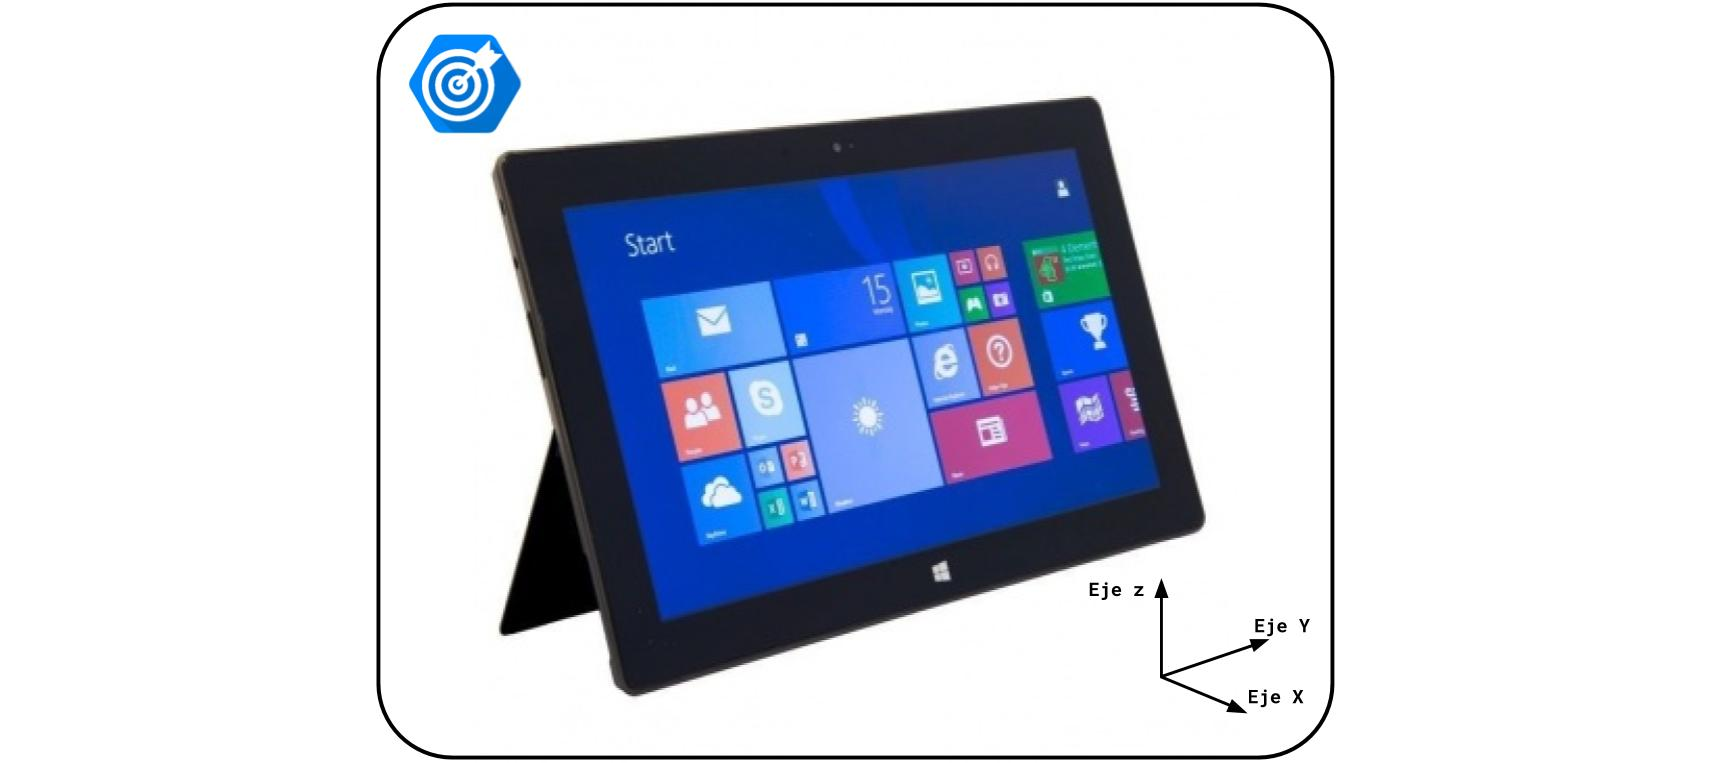
\includegraphics[width=1\textwidth]{figuras/Imagenes_Conclusion/orientacion_tablet.jpg}
	\caption{Sistema de referencia para los grados de libertad de orientación}
	\label{fig:Conclusiones:orientacion_tablet}
	\immagesource{Imagen del fabricante editada por el autor}
\end{figure}

\subsection{Mejoras generales}

Una segunda iteración podría centrarse también en identificar diferentes mejoras posibles a robustecer que hayan pasado desapercibidas en los test realizados para los diferentes aspectos del diseño.